\documentclass[12pt,english]{scrartcl}

\usepackage{amsmath,amssymb}
%\usepackage[amssymb]{SIunits}
\usepackage{babel}
\usepackage[latin1]{inputenc}
\usepackage{graphicx}
\usepackage{color}
\usepackage{url}


\begin{document}

\begin{center}
\textbf{\begin{LARGE}KOGW-PM-KNP:\\ \vspace{3mm} Tutorial 9 - Grasping
\end{LARGE}}
\end{center}

This tutorial deals with object manipulation performance. The paper by Wunsch et al., (2014) studies second-order motion planning in children of different age groups and compares it to performance in human adults and in cotton-top tamarin monkeys (see Fig. \ref{fig:tamarin}). Please read the paper carefully. Answer the following questions which should help you to evaluate the findings. Please work in pairs. 
 
\begin{figure}[htbp]
\begin{center}
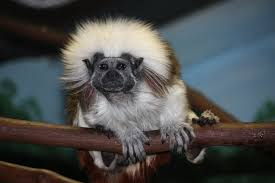
\includegraphics[width = 0.5\textwidth]{../../Slides/figs/l9/cotton_top_tamarin.jpg}
\end{center}
\caption{Cotton-top tamarin monkey
\label{fig:tamarin}}
\end{figure}

\begin{enumerate}
 \item What is involved in motor planning? What is meant by second-order motor planning? What is the end-state comfort (ESC) effect?

 \color{blue}
 \begin{itemize}
 \item selection of one particular sequence of motor movements from a nearly infinite set of possible movements
 \item consideration of subsequent actions for selection of movements
 \item organization of motor actions in a way that ensure greater control at the end of the movement
 \end{itemize}
  \color{black}

 \item How is ESC studied experimentally? What is the evidence as to when ESC effects emerge during development?

 \color{blue}
 \begin{itemize}
 \item turn over a glass and fill it with water
 \item ESC reliably emerge between 3 and 8y of age
 \item adult-like performance not before the age of 10
 \end{itemize}
  \color{black}

 \item How do monkeys (cotton-top tamarins and lemurs) perform on these tasks? Why is their performance surprising?

 \color{blue}
 \begin{itemize}
 \item tamarins and lemurs use an inverted, thumb-down grasping posture
 \item tamarins are non-tool using species whereas children do use tools, counterintuitive that tamarins more similar to adults than to children 
 \end{itemize}
  \color{black}

\item What factor do the authors suggest to be potentially responsible for the putative discrepancy?
 \color{blue}
 \begin{itemize}
 \item in the overturned-glass-task used with children the task tends to be oriented towards an external goal 
 \item tamarin monkeys were grasping for a cup (upright or overturned) that contained a food reward
 \item self-directed motor planning tasks may elicit more effective motor plannign than externally-oriented tasks, consequences of actions more obvious to participants
 \end{itemize}
  \color{black}

\item What hypothesis did the authors test in the present experiment? What is the alternative hypothesis?

 \color{blue}
 \begin{itemize}
 \item \textit{If} the discrepancy in findings between the tamarin study and previous studies with children relates to the orientation of subsequent actions,  \textit{then} there should be evidence for reliable second-order-planning in some children when the children are tested with a more self-directed task
\item If the mechanism underlying the cross-species difference is biomechanical in nature, then results with a self-directed task should be comparable to previous results
 \end{itemize}
  \color{black}

\item Describe the present experiment, design, independent, dependent, control variables

 \color{blue}
 \begin{itemize}
 \item independent variables: 
 \begin{itemize}
  \item age: preschool (5y), young school (7.7y), older school (9.8y), adults (26.8y)
  \item cup orientation: upright, inverted
 \end{itemize}
 
\item dependent variable: hand position: upright, inverted
\item between subject design
\item control variable: starting position of cup orientation = counterbalanced across participants
 \end{itemize}
  \color{black}

\item What is the main result of this study?

 \color{blue}
 \begin{itemize}
 \item Figure 2: participants showing end-state comfort in at least three out of four trials under the two conditions
 \item upright-cup: all participants choose a thumb-up grasp position
 \item inverted-cup: none of the preschoolers, 13\% of the younger, 58\% of the older school children, 87\% of the adults
 \end{itemize}
  \color{black}


\item What do the authors conclude from their results? What kind of explanations do they offer? What do you find plausible?
 \color{blue}
 \begin{itemize}
 \item no evidence of ESC in the group of preschool children, support of previous findings with respect to the development of ESC
 \item tamarins behave more like human adults than do young children
 \item tamarins do exhibit ESC but do not use tools in the wild
 \item children's \textit{perception of comfort} might be different from that of adults, children perceive postures at both ends of their supination or pronation range as less awkward
 \item morphological constraint hypothesis: less dexterous species demonstrate more second-order motion planning because they have fewer means to compensate for initially suboptimal grip - consistent with feedforward internal model of the extended motor system which predicts sensory outcomes prior to the execution of motor actions

 
 
 \end{itemize}
  \color{black}

\end{enumerate}

\end{document}
